\section*{Acknowledgements}
The possibility that the Yang--Mills gradient flow (or the Wilson flow) can be
useful for defining the energy--momentum tensor in lattice gauge theory was
originally suggested to me by Etsuko Itou. I would like to thank her for
enlightening discussions. I would also like to thank Martin L\"uscher for a
clarifying remark on the precise meaning of~Eq.~\eqref{eq:(3.8)}.
I am grateful to Hiroki Makino for his help in finding errors in the one-loop
calculation in previous versions of the preset paper.
This work is supported in part by a Grant-in-Aid for Scientific
Research~23540330.

\appendix

\section{One-loop calculation of coefficient functions}
\label{sec:5}
For calculational convenience, we define the coefficient functions $F(t)$
and~$G(t)$ by
\begin{align}
   &G_{\mu\rho}^a(t,x)G_{\nu\rho}^a(t,x)
   -\left\langle G_{\mu\rho}^a(t,x)G_{\nu\rho}^a(t,x)\right\rangle
\notag\\
   &\qquad{}
   =F(t)\left\{F_{\mu\rho}^aF_{\nu\rho}^a\right\}_R(x)
   +G(t)\delta_{\mu\nu}\left\{F_{\rho\sigma}^aF_{\rho\sigma}^a\right\}_R(x)
   +O(t).
\label{eq:(5.1)}
\end{align}
Equation~\eqref{eq:(3.5)} then becomes (for $D=4$),
\begin{align}
   U_{\mu\nu}(t,x)
   &=F(t)\left[
   \left\{F_{\mu\rho}^aF_{\nu\rho}^a\right\}_R(x)
   -\frac{1}{4}\delta_{\mu\nu}
   \delta_{\rho\lambda}\left\{F_{\rho\sigma}^aF_{\lambda\sigma}^a\right\}_R(x)
   \right]
   +O(t)
\notag\\
   &=F(t)\left[
   \left\{F_{\mu\rho}^aF_{\nu\rho}^a\right\}_R(x)
   -\frac{1}{4}\delta_{\mu\nu}
   \left(1-\frac{\beta}{2g}\right)
   \left\{F_{\rho\sigma}^aF_{\rho\sigma}^a\right\}_R(x)
   \right]
   +O(t),
\label{eq:(5.2)}
\end{align}
where we have used Eq.~\eqref{eq:(2.19)}. Rewriting this in favor of the
energy--momentum tensor~\eqref{eq:(2.12)} with Eqs.~\eqref{eq:(2.13)}
and~\eqref{eq:(2.14)}, we have
\begin{align}
   U_{\mu\nu}(t,x)
   &=F(t)\left[
   \left\{F_{\mu\rho}^aF_{\nu\rho}^a\right\}_R(x)
   -\frac{1}{4}\delta_{\mu\nu}
   \delta_{\rho\lambda}\left\{F_{\rho\sigma}^aF_{\lambda\sigma}^a\right\}_R(x)
   \right]
   +O(t)
\notag\\
   &=F(t)\left[
   g^2\left\{T_{\mu\nu}\right\}_R(x)
   +\frac{\beta}{8g}\delta_{\mu\nu}
   \left\{F_{\rho\sigma}^aF_{\rho\sigma}^a\right\}_R(x)
   \right]
   +O(t).
\label{eq:(5.3)}
\end{align}
Comparison with~Eq.~\eqref{eq:(3.7)} then shows
\begin{equation}
   c_T(t)=g^2F(t),\qquad c_S(t)=\frac{\beta}{2g}F(t).
\label{eq:(5.4)}
\end{equation}

Similarly, for~Eq.~\eqref{eq:(3.8)},
\begin{align}
   E(t,x)
   &=\left\langle E(t,x)\right\rangle
   +\frac{1}{4}F(t)\delta_{\rho\lambda}
   \left\{F_{\rho\sigma}^aF_{\lambda\sigma}^a\right\}_R(x)
   +G(t)\left\{F_{\rho\sigma}^aF_{\rho\sigma}^a\right\}_R(x)
   +O(t)
\notag\\
   &=\left[
   \left(1-\frac{\beta}{2g}\right)F(t)+4G(t)\right]
   \left\{\frac{1}{4}F_{\rho\sigma}^aF_{\rho\sigma}^a\right\}_R(x)
   +O(t),
\label{eq:(5.5)}
\end{align}
and therefore
\begin{equation}
   c_E(t)=\left(1-\frac{\beta}{2g}\right)F(t)+4G(t).
\label{eq:(5.6)}
\end{equation}
This implies, for the ratio~\eqref{eq:(4.23)},
\begin{align}
   \frac{c_S(t)}{c_E(t)}
   &=\frac{\beta}{2g}\frac{1}{1-\frac{\beta}{2g}+4G(t)/F(t)}
\notag\\
   &=-\frac{b_0}{2}g^2
   \left\{1+2b_0g^2\left[-\frac{1}{4}+\frac{b_1}{2b_0^2}\right]
   -4G(t)+O(g^4)\right\}.
\label{eq:(5.7)}
\end{align}

To find the coefficient functions $F(t)$ and~$G(t)$ in~Eq.~\eqref{eq:(5.1)}, we
consider the correlation function
\begin{equation}
   \left\langle G_{\mu\rho}^a(t,x)G_{\nu\rho}^a(t,x)
   A_\kappa^i(w)A_\omega^j(v)\right\rangle.
\label{eq:(5.8)}
\end{equation}
For~$O(g_0^2)$, there are $17$ flow-line Feynman diagrams
(Figs.~\ref{fig:1}--\ref{fig:17}) that contribute to this correlation function.
In the figures, gauge potentials at the flow time~$t$, $B_\mu(t,x)$, are
represented by small filled squares; the open circle denotes the flow-time
vertex and the full circle is the conventional vertex in the Yang-Mills theory.
We refer the reader to~Ref.~\cite{Luscher:2011bx} for the details of the
Feynman rules for flow-line diagrams.

To read off the coefficient functions $F(t)$ and~$G(t)$ in~Eq.~\eqref{eq:(5.1)}
from the correlation function~\eqref{eq:(5.8)}, we consider the vertex
functions, i.e., amputated diagrams in which the external propagators of the
original Yang--Mills theory are truncated. Therefore, Figs.~\ref{fig:10},
\ref{fig:12} and~\ref{fig:17}, which provide only the conventional wave
function renormalization, should be omitted in the computation of $F(t)$
and~$G(t)$.\footnote{More precisely, these diagrams are different from
conventional Feynman diagrams in that the propagators carry an additional
factor $e^{-tp^2}$ (in the Feynman gauge), where $p$ is the external momentum.
This factor is, however, irrelevant in the present computation of the
coefficients of operators with the lowest number of derivatives.} On the other
hand, the flow-line propagators~\cite{Luscher:2011bx}, the arrowed straight
lines in the diagrams, should not be truncated because these are not
propagators in the quantum field theory but instead represent time evolution
along the flow time.

\begin{figure}
\centering
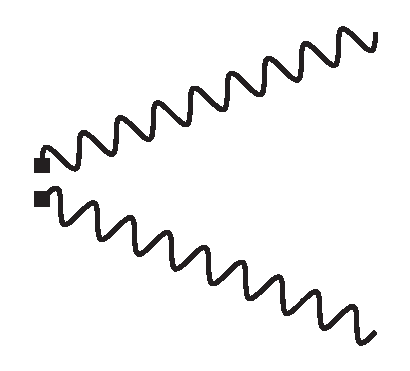
\includegraphics[width=3cm,clip]{images/diagram_1}
\caption{}
\label{fig:1}
\end{figure}

\begin{figure}
\centering
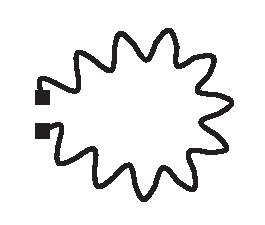
\includegraphics[width=3cm,clip]{images/diagram_2}
\caption{}
\label{fig:2}
\end{figure}

\begin{figure}
\begin{minipage}{0.3\hsize}
\begin{center}
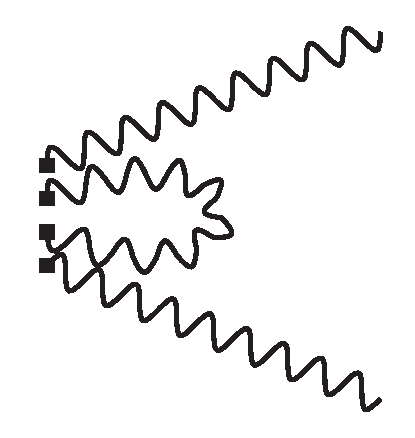
\includegraphics[width=3cm,clip]{images/diagram_3}
\caption{}
\label{fig:3}
\end{center}
\end{minipage}
\begin{minipage}{0.3\hsize}
\begin{center}
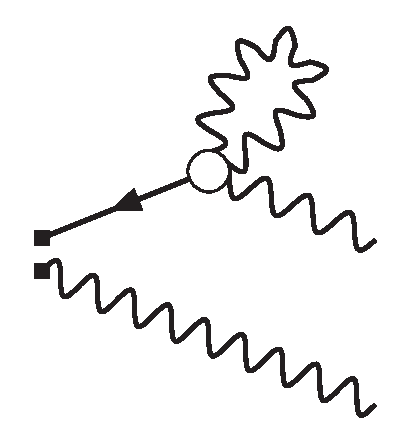
\includegraphics[width=3cm,clip]{images/diagram_4}
\caption{}
\label{fig:4}
\end{center}
\end{minipage}
\begin{minipage}{0.3\hsize}
\begin{center}
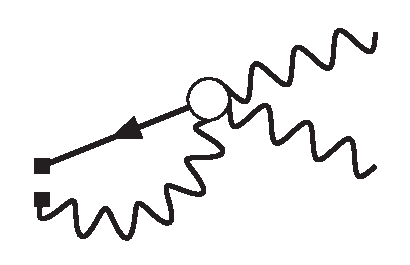
\includegraphics[width=3cm,clip]{images/diagram_5}
\caption{}
\label{fig:5}
\end{center}
\end{minipage}
\end{figure}

\begin{figure}
\begin{minipage}{0.3\hsize}
\begin{center}
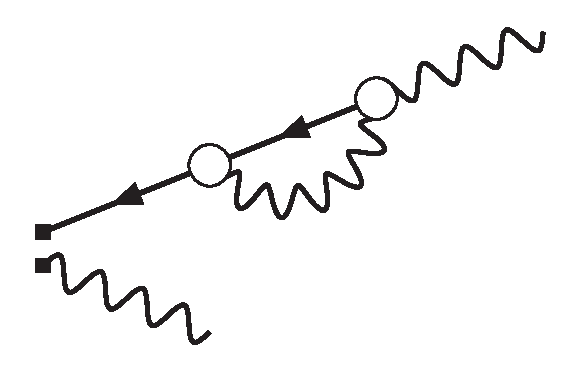
\includegraphics[width=4cm,clip]{images/diagram_6}
\caption{}
\label{fig:6}
\end{center}
\end{minipage}
\begin{minipage}{0.3\hsize}
\begin{center}
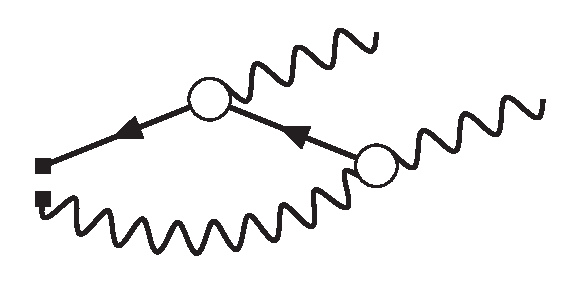
\includegraphics[width=4cm,clip]{images/diagram_7}
\caption{}
\label{fig:7}
\end{center}
\end{minipage}
\begin{minipage}{0.3\hsize}
\begin{center}
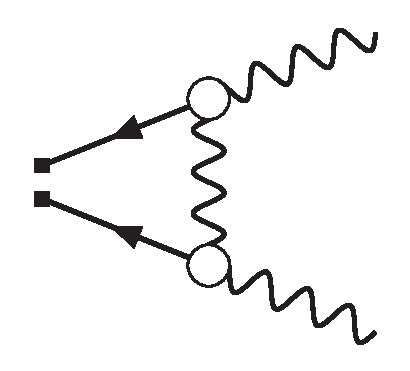
\includegraphics[width=3cm,clip]{images/diagram_8}
\caption{}
\label{fig:8}
\end{center}
\end{minipage}
\end{figure}

\begin{figure}
\begin{minipage}{0.3\hsize}
\begin{center}
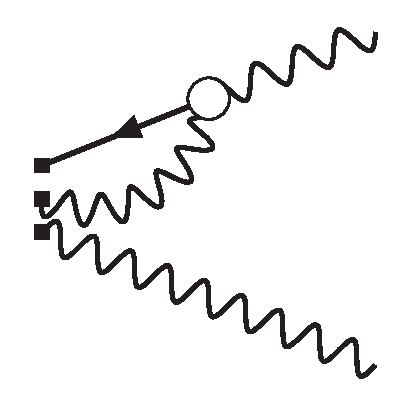
\includegraphics[width=3cm,clip]{images/diagram_9}
\caption{}
\label{fig:9}
\end{center}
\end{minipage}
\begin{minipage}{0.3\hsize}
\begin{center}
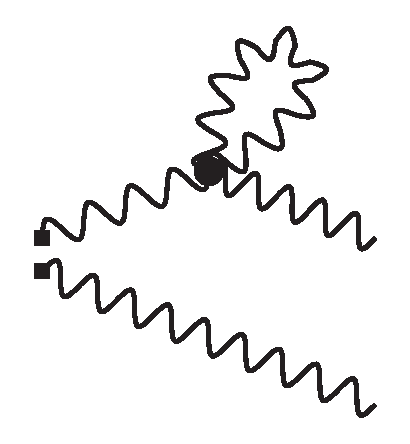
\includegraphics[width=3cm,clip]{images/diagram_10}
\caption{}
\label{fig:10}
\end{center}
\end{minipage}
\begin{minipage}{0.3\hsize}
\begin{center}
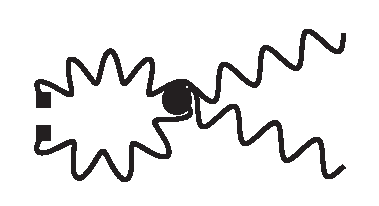
\includegraphics[width=3cm,clip]{images/diagram_11}
\caption{}
\label{fig:11}
\end{center}
\end{minipage}
\end{figure}

\begin{figure}
\begin{minipage}{0.3\hsize}
\begin{center}
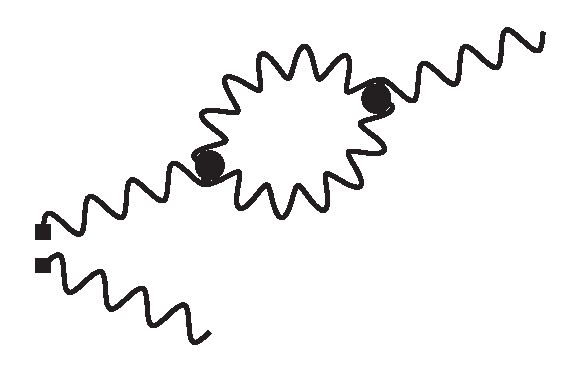
\includegraphics[width=4cm,clip]{images/diagram_12}
\caption{}
\label{fig:12}
\end{center}
\end{minipage}
\begin{minipage}{0.3\hsize}
\begin{center}
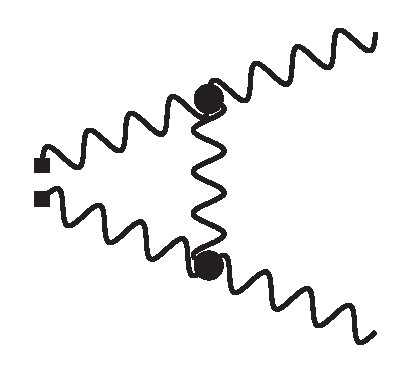
\includegraphics[width=3cm,clip]{images/diagram_13}
\caption{}
\label{fig:13}
\end{center}
\end{minipage}
\begin{minipage}{0.3\hsize}
\begin{center}
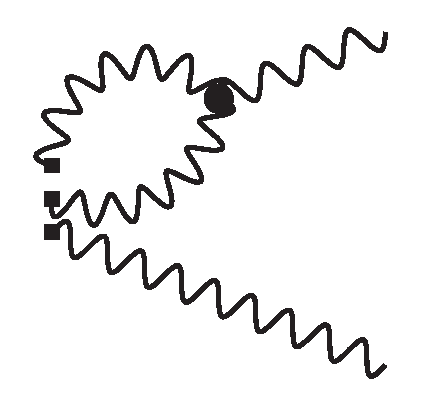
\includegraphics[width=3cm,clip]{images/diagram_14}
\caption{}
\label{fig:14}
\end{center}
\end{minipage}
\end{figure}

\begin{figure}
\begin{minipage}{0.3\hsize}
\begin{center}
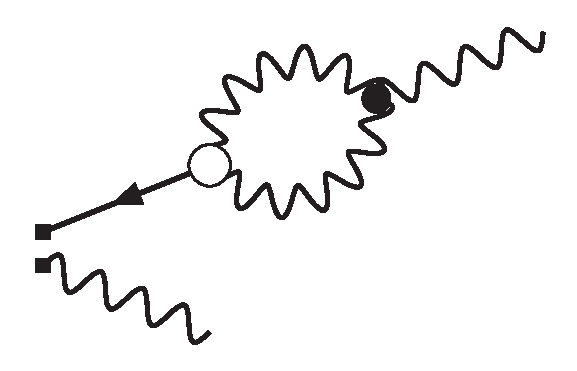
\includegraphics[width=4cm,clip]{images/diagram_15}
\caption{}
\label{fig:15}
\end{center}
\end{minipage}
\begin{minipage}{0.3\hsize}
\begin{center}
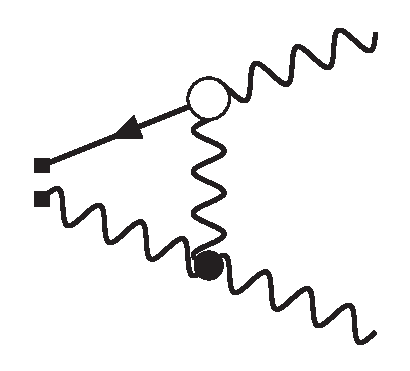
\includegraphics[width=3cm,clip]{images/diagram_16}
\caption{}
\label{fig:16}
\end{center}
\end{minipage}
\begin{minipage}{0.3\hsize}
\begin{center}
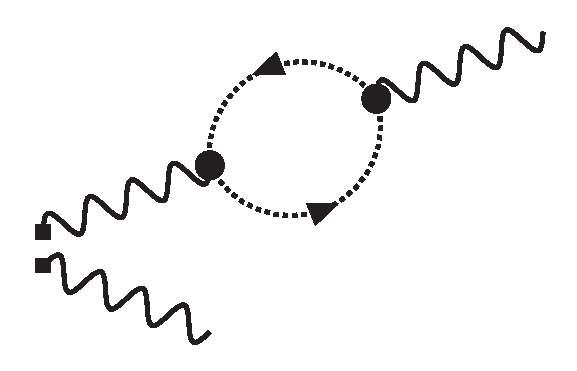
\includegraphics[width=4cm,clip]{images/diagram_17}
\caption{}
\label{fig:17}
\end{center}
\end{minipage}
\end{figure}

The tree-level contribution to the vertex function is
\begin{align}
   \text{Fig.~\ref{fig:1}}
   &=\delta_{\rho\sigma}\left[
   \int_{p,q}\,e^{i(p+q)x}\Tilde{A}_\rho^a(p)\Tilde{A}_\sigma^a(q)
   e^{-tp^2}e^{-tq^2}ip_\mu iq_\nu
   \pm(\mu\leftrightarrow\rho,\nu\leftrightarrow\sigma)\right]
\notag\\
   &=F_{\mu\rho}^a(x)F_{\nu\sigma}^a(x)+O(t),
\label{eq:(5.9)}
\end{align}
where
\begin{equation}
   A_\mu(x)=\int_pe^{ipx}\Tilde{A}_\mu(p),\qquad
   \int_p\equiv\int\frac{d^Dp}{(2\pi)^D},
\label{eq:(5.10)}
\end{equation}
and, here and in what follows, the alternating-sign symbol implies
\begin{equation}
   t_{\mu\rho\nu\sigma}\pm(\mu\leftrightarrow\rho,\nu\leftrightarrow\sigma)
   \equiv
   t_{\mu\rho\nu\sigma}-t_{\rho\mu\nu\sigma}-t_{\mu\rho\sigma\nu}
   +t_{\rho\mu\sigma\nu}.
\label{eq:(5.11)}
\end{equation}
This tree-level result was used in obtaining~Eq.~\eqref{eq:(4.20)}.

The vacuum expectation value in the lowest order is
\begin{align}
   \text{Fig.~\ref{fig:2}}&=g_0^2\delta^{aa}\delta_{\rho\sigma}
   \left[\int_\ell\frac{1}{\ell^2}\,e^{-2t\ell^2}
   \ell_\mu\ell_\nu\delta_{\rho\sigma}
   \pm(\mu\leftrightarrow\rho,\nu\leftrightarrow\sigma)\right]
\notag\\
   &=\frac{3}{128\pi^2}(N^2-1)
   g_0^2\frac{1}{t^2}\delta_{\mu\nu}.
\label{eq:(5.12)}
\end{align}

Now, as an example of the computation of one-loop flow-line Feynman diagrams,
we briefly illustrate the computation of~Fig~\ref{fig:13}. A straightforward
application of the Feynman rules in~Ref.~\cite{Luscher:2011bx} in the
``Feynman gauge'' in which the gauge parameters are taken
as~$\lambda_0=\alpha_0=1$, yields the expression,
% [Intermediate expressions for Figs. 3-17 present as comments in the arXiv
%  source are omitted here; see the original source file
%  EM_extended_ptep_ver6.tex.]
\begin{align}
   \text{Fig.~\ref{fig:13}}
   &=Ng_0^2\delta_{\rho\sigma}\biggl(
   \int_{p,q}\,e^{i(p+q)x}\Tilde{A}_\alpha^b(p)\Tilde{A}_\beta^c(q)
\notag\\
   &\qquad{}\times
   \int_\ell
   \frac{1}{(p+\ell)^2}\frac{1}{\ell^2}\frac{1}{(q-\ell)^2}\,
   e^{-t(p+\ell)^2}e^{-t(q-\ell)^2}
\notag\\
   &\qquad\qquad{}\times
   i(p+\ell)_\mu i(q-\ell)_\nu
\notag\\
   &\qquad\qquad{}\times
   \left[\delta_{\rho\lambda}(-p-2\ell)_\alpha
   +\delta_{\lambda\alpha}(\ell-p)_\rho
   +\delta_{\alpha\rho}(2p+\ell)_\lambda\right]
\notag\\
   &\qquad\qquad{}\times
   \left[\delta_{\lambda\sigma}(-2\ell+q)_\beta
   +\delta_{\sigma\beta}(-2q+\ell)_\lambda
   +\delta_{\beta\lambda}(q+\ell)_\sigma\right]
\notag\\
   &\qquad\qquad\qquad{}\pm(\mu\leftrightarrow\rho,\nu\leftrightarrow\sigma)
   \biggr).
\label{eq:(5.13)}
\end{align}

To find the coefficients $F(t)$ and~$G(t)$ in~Eq.~\eqref{eq:(5.1)}, we write
this vertex function as
\begin{equation}
   \int_{p,q}\,e^{i(p+q)x}\Tilde{A}_\alpha^a(p)\Tilde{A}_\beta^a(q)
   M_{\mu\nu,\alpha\beta}(p,q),
\label{eq:(5.14)}
\end{equation}
and find the coefficients of
\begin{equation}
   -p_\mu q_\nu\delta_{\alpha\beta}
\label{eq:(5.15)}
\end{equation}
and
\begin{equation}
%   -2p\cdot q\delta_{\mu\nu}\delta_{\alpha\beta},
   -4p\cdot q\delta_{\mu\nu}\delta_{\alpha\beta},
\label{eq:(5.16)}
\end{equation}
respectively, in~$M_{\mu\nu,\alpha\beta}(p,q)$. For this, we first exponentiate
the denominators in~Eq.~\eqref{eq:(5.13)} by using
\begin{equation}
   \frac{1}{(p+\ell)^2}\frac{1}{(q-\ell)^2}
   =\int_0^\infty d\xi\,\int_0^\infty d\eta\,e^{-\xi(p+\ell)^2}e^{-\eta(q-\ell)^2}.
\label{eq:(5.17)}
\end{equation}
We then simply expand the integrand with respect to the external momenta $p$
and~$q$ to $O(p,q)$. The flow-time evolution factor~$e^{-2t\ell^2}$ in the
integrand makes the integral~\eqref{eq:(5.13)} UV finite for any dimension~$D$.
On the other hand, there always exists a complex domain of~$D$ such that the
integral is infrared finite; this provides the analytic continuation of the
integral such that
\begin{align}
   &\int_\ell\frac{1}{\ell^2}\,
   e^{-\alpha\ell^2}=\frac{1}{(4\pi)^{D/2}}\frac{1}{D/2-1}\alpha^{-D/2+1},
\label{eq:(5.18)}
\\
   &\int_\ell\frac{1}{\ell^2}\,e^{-\alpha\ell^2}\ell_\mu\ell_\nu
   =\frac{1}{(4\pi)^{D/2}}\frac{1}{D}\alpha^{-D/2}\delta_{\mu\nu},
\label{eq:(5.19)}
\\
   &\int_\ell\frac{1}{\ell^2}\,e^{-\alpha\ell^2}
   \ell_\mu\ell_\nu\ell_\rho\ell_\sigma
   =\frac{1}{(4\pi)^{D/2}}\frac{1}{2(D+2)}\alpha^{-D/2-1}
   \left(
   \delta_{\mu\nu}\delta_{\rho\sigma}
   +\delta_{\mu\rho}\delta_{\nu\sigma}
   +\delta_{\mu\sigma}\delta_{\nu\rho}
   \right),
\label{eq:(5.20)}
\\
   &\int_\ell\frac{1}{\ell^2}\,e^{-\alpha\ell^2}
   \ell_\mu\ell_\nu\ell_\rho\ell_\sigma\ell_\alpha\ell_\beta
\notag\\
   &=\frac{1}{(4\pi)^{D/2}}\frac{1}{4(D+4)}\alpha^{-D/2-2}
   \left(
   \delta_{\mu\nu}\delta_{\rho\sigma}\delta_{\alpha\beta}
   +\text{$14$ permutations}\right).
\label{eq:(5.21)}
\end{align}
Then it is straightforward to find the coefficients of Eqs.~\eqref{eq:(5.15)}
and~\eqref{eq:(5.16)}, which directly make a contribution to the functions
$F(t)$ and~$G(t)$.

\begin{table}
\caption{The contributions of each flow-line Feynman diagram (in the Feynman
gauge) to the coefficients of Eqs.~\eqref{eq:(5.15)} and~\eqref{eq:(5.16)},
respectively, in the unit of~Eq.~\eqref{eq:(5.22)}. These correspond to the
coefficient functions $F(t)$ and~$G(t)$ in~Eq.~\eqref{eq:(5.1)}.
The numbers with~$*$ are corrected from previous versions of the present paper.
}
\label{table:1}
\begin{center}
\renewcommand{\arraystretch}{2.2}
\setlength{\tabcolsep}{12pt}
\begin{tabular}{crr}
\toprule
 & \multicolumn{1}{c}{$F(t)$}
 & \multicolumn{1}{c}{$G(t)$} \\
\midrule
Fig.~\ref{fig:3}  & $0$ & $0$ \\
Fig.~\ref{fig:4}  & $-3\dfrac{1}{\epsilon}-3\ln(8\pi t)-1$ & $0$ \\
Fig.~\ref{fig:5}  & $-\dfrac{7}{36}$ & $-\dfrac{49}{144}$ \\
Fig.~\ref{fig:6}  & $2\dfrac{1}{\epsilon}+2\ln(8\pi t)-\dfrac{1}{2}$ & $0$ \\
Fig.~\ref{fig:7}  & $\dfrac{19}{288}$ & $\dfrac{121}{384}$ \\
%Fig.~\ref{fig:8}  & $\dfrac{47}{96}$ & $\dfrac{53}{128}$ \\
Fig.~\ref{fig:8}  & $\dfrac{35}{96}^*$ & $\dfrac{143}{384}^*$ \\
Fig.~\ref{fig:9}  & $-\dfrac{25}{8}$ & $0$\\
%Fig.~\ref{fig:10} & --- & --- \\
Fig.~\ref{fig:11}  & $\dfrac{1}{3}\dfrac{1}{\epsilon}+\dfrac{1}{3}\ln(8\pi t)-\dfrac{17}{36}$ & $\dfrac{7}{12}\dfrac{1}{\epsilon}+\dfrac{7}{12}\ln(8\pi t)+\dfrac{1}{144}$\\
%Fig.~\ref{fig:12} & --- & --- \\
Fig.~\ref{fig:13}  & $-\dfrac{5}{3}\dfrac{1}{\epsilon}-\dfrac{5}{3}\ln(8\pi t)+\dfrac{25}{36}$ & $-\dfrac{3}{2}\dfrac{1}{\epsilon}-\dfrac{3}{2}\ln(8\pi t)-\dfrac{29}{16}$\\
Fig.~\ref{fig:14} & $3\dfrac{1}{\epsilon}+3\ln(8\pi t)+3$ & $0$ \\
Fig.~\ref{fig:15}  & $3\dfrac{1}{\epsilon}+3\ln(8\pi t)+\dfrac{5}{2}$ & $0$ \\
%Fig.~\ref{fig:16}  & $\dfrac{7}{4}$ & $\dfrac{31}{24}$ \\
Fig.~\ref{fig:16}  & $1^*$ & $\dfrac{31}{24}$ \\
%Fig.~\ref{fig:17} & --- & --- \\
$Z$~factors & $-\dfrac{11}{3}\dfrac{1}{\epsilon}$ & $\dfrac{11}{12}\dfrac{1}{\epsilon}$ \\
\bottomrule
\end{tabular}
\end{center}
\end{table}

In Table~\ref{table:1}, we summarize the contribution of each diagram
computed in the above method in the unit of
\begin{equation}
   \frac{1}{16\pi^2}Ng_0^2.
\label{eq:(5.22)}
\end{equation}
In the last line of the table, ``$Z$~factors'' implies the contributions of the
one-loop operator renormalization factors, $Z_T$~\eqref{eq:(2.13)} and
$Z_M$~\eqref{eq:(2.22)}, through the tree-level diagram, Eq.~\eqref{eq:(5.9)}
(recall Eq.~\eqref{eq:(2.10)}). We see that those operator renormalization
factors precisely cancel the residues of~$1/\epsilon$ and make the coefficients
$F(t)$ and~$G(t)$ finite; this is precisely what we expect from the general
argument. From the results in the table, we then have
\begin{align}
   F(t)&=1+2b_0g^2
   \left[\ln(\sqrt{8t}\mu)+\ln\sqrt{\pi}+\frac{7}{22}\right],
\label{eq:(5.23)}
\\
   G(t)&=-\frac{1}{2}b_0g^2
   \left[\ln(\sqrt{8t}\mu)+\ln\sqrt{\pi}+\frac{1}{11}\right].
\label{eq:(5.24)}
\end{align}
Finally, comparison with the formulas~\eqref{eq:(5.4)}, \eqref{eq:(5.7)},
\eqref{eq:(4.21)} and~\eqref{eq:(4.23)} shows the results quoted
in~Sect.~\ref{sec:4}, Eqs.~\eqref{eq:(4.30)} and~\eqref{eq:(4.31)}. Note that
the coefficients of $\ln(\sqrt{8t}\mu)$ in the explicit one-loop calculation
(Eqs.~\eqref{eq:(5.23)} and~\eqref{eq:(5.24)}) are in agreement with those by
the general argument on the basis of the renormalization group equations and
the trace anomaly (Eqs.~\eqref{eq:(4.21)} and~\eqref{eq:(4.23)}). This
agreement provides a consistency check for our one-loop calculation and
supports the correctness of our reasoning.

\begin{thebibliography}{00}

%\cite{Nielsen:1980rz}
\bibitem{Nielsen:1980rz}
  H.~B.~Nielsen and M.~Ninomiya,
  Nucl.\ Phys.\ B {\bf 185}, 20 (1981)
  [Erratum-ibid.\ B {\bf 195}, 541 (1982)].
  %%CITATION = NUPHA,B185,20;%%

%\cite{Nielsen:1981xu}
\bibitem{Nielsen:1981xu}
  H.~B.~Nielsen and M.~Ninomiya,
  Nucl.\ Phys.\ B {\bf 193}, 173 (1981).
  %%CITATION = NUPHA,B193,173;%%

%\cite{Dondi:1976tx}
\bibitem{Dondi:1976tx}
  P.~H.~Dondi and H.~Nicolai,
  Nuovo Cim.\ A {\bf 41}, 1 (1977).
  %%CITATION = NUCIA,A41,1;%%

%\cite{Kaplan:1992bt}
\bibitem{Kaplan:1992bt}
  D.~B.~Kaplan,
  Phys.\ Lett.\ B {\bf 288}, 342 (1992)
  [hep-lat/9206013].
  %%CITATION = HEP-LAT/9206013;%%

%\cite{Neuberger:1997fp}
\bibitem{Neuberger:1997fp}
  H.~Neuberger,
  Phys.\ Lett.\ B {\bf 417}, 141 (1998)
  [hep-lat/9707022].
  %%CITATION = HEP-LAT/9707022;%%

%\cite{Hasenfratz:1997ft}
\bibitem{Hasenfratz:1997ft}
  P.~Hasenfratz,
  Nucl.\ Phys.\ Proc.\ Suppl.\  {\bf 63}, 53 (1998)
  [hep-lat/9709110].
  %%CITATION = HEP-LAT/9709110;%%

%\cite{Hasenfratz:1998ri}
\bibitem{Hasenfratz:1998ri}
  P.~Hasenfratz, V.~Laliena and F.~Niedermayer,
  Phys.\ Lett.\ B {\bf 427}, 125 (1998)
  [hep-lat/9801021].
  %%CITATION = HEP-LAT/9801021;%%

%\cite{Neuberger:1998wv}
\bibitem{Neuberger:1998wv}
  H.~Neuberger,
  Phys.\ Lett.\ B {\bf 427}, 353 (1998)
  [hep-lat/9801031].
  %%CITATION = HEP-LAT/9801031;%%

%\cite{Hasenfratz:1998jp}
\bibitem{Hasenfratz:1998jp}
  P.~Hasenfratz,
  Nucl.\ Phys.\ B {\bf 525}, 401 (1998)
  [hep-lat/9802007].
  %%CITATION = HEP-LAT/9802007;%%

%\cite{Luscher:1998pqa}
\bibitem{Luscher:1998pqa}
  M.~L\"uscher,
  Phys.\ Lett.\ B {\bf 428}, 342 (1998)
  [hep-lat/9802011].
  %%CITATION = HEP-LAT/9802011;%%

%\cite{Niedermayer:1998bi}
\bibitem{Niedermayer:1998bi}
  F.~Niedermayer,
  Nucl.\ Phys.\ Proc.\ Suppl.\  {\bf 73}, 105 (1999)
  [hep-lat/9810026].
  %%CITATION = HEP-LAT/9810026;%%

%\cite{Ginsparg:1981bj}
\bibitem{Ginsparg:1981bj}
  P.~H.~Ginsparg and K.~G.~Wilson,
  Phys.\ Rev.\ D {\bf 25}, 2649 (1982).
  %%CITATION = PHRVA,D25,2649;%%

%\cite{Kato:2008sp}
\bibitem{Kato:2008sp}
  M.~Kato, M.~Sakamoto and H.~So,
  JHEP {\bf 0805}, 057 (2008)
  [arXiv:0803.3121 [hep-lat]].
  %%CITATION = ARXIV:0803.3121;%%

%\cite{Callan:1970ze}
\bibitem{Callan:1970ze}
  C.~G.~Callan, Jr., S.~R.~Coleman and R.~Jackiw,
  Annals Phys.\  {\bf 59}, 42 (1970).
  %%CITATION = APNYA,59,42;%%

%\cite{Coleman:1970je}
\bibitem{Coleman:1970je}
  S.~R.~Coleman and R.~Jackiw,
  Annals Phys.\  {\bf 67}, 552 (1971).
  %%CITATION = APNYA,67,552;%%

%\cite{Caracciolo:1988hc}
\bibitem{Caracciolo:1988hc}
  S.~Caracciolo, G.~Curci, P.~Menotti and A.~Pelissetto,
  Nucl.\ Phys.\ B {\bf 309}, 612 (1988).
  %%CITATION = NUPHA,B309,612;%%

%\cite{Caracciolo:1989pt}
\bibitem{Caracciolo:1989pt}
  S.~Caracciolo, G.~Curci, P.~Menotti and A.~Pelissetto,
  Annals Phys.\  {\bf 197}, 119 (1990).
  %%CITATION = APNYA,197,119;%%

%\cite{Suzuki:2013gi}
\bibitem{Suzuki:2013gi}
  H.~Suzuki,
  Nucl.\ Phys.\ B {\bf 868}, 459 (2013)
  [arXiv:1209.2473 [hep-lat]].
  %%CITATION = ARXIV:1209.2473;%%

%\cite{Suzuki:2012wx}
\bibitem{Suzuki:2012wx}
  H.~Suzuki,
  Phys.\ Lett.\ B {\bf 719}, 435 (2013)
  [arXiv:1209.5155 [hep-lat]].
  %%CITATION = ARXIV:1209.5155;%%

%\cite{Bochicchio:1985xa}
\bibitem{Bochicchio:1985xa}
  M.~Bochicchio, L.~Maiani, G.~Martinelli, G.~C.~Rossi and M.~Testa,
  Nucl.\ Phys.\ B {\bf 262}, 331 (1985).
  %%CITATION = NUPHA,B262,331;%%

%\cite{Fujikawa:1980rc}
\bibitem{Fujikawa:1980rc}
  K.~Fujikawa,
  Phys.\ Rev.\ D {\bf 23}, 2262 (1981).
  %%CITATION = PHRVA,D23,2262;%%

%\cite{Fujikawa:2004cx}
\bibitem{Fujikawa:2004cx}
  K.~Fujikawa and H.~Suzuki,
  ``Path integrals and quantum anomalies,''
  Oxford, UK: Clarendon (2004) 284 p

%\cite{Crewther:1972kn}
\bibitem{Crewther:1972kn}
  R.~J.~Crewther,
  Phys.\ Rev.\ Lett.\  {\bf 28}, 1421 (1972).
  %%CITATION = PRLTA,28,1421;%%

%\cite{Chanowitz:1972vd}
\bibitem{Chanowitz:1972vd}
  M.~S.~Chanowitz and J.~R.~Ellis,
  Phys.\ Lett.\ B {\bf 40}, 397 (1972).
  %%CITATION = PHLTA,B40,397;%%

%\cite{Adler:1976zt}
\bibitem{Adler:1976zt}
  S.~L.~Adler, J.~C.~Collins and A.~Duncan,
  Phys.\ Rev.\ D {\bf 15}, 1712 (1977).
  %%CITATION = PHRVA,D15,1712;%%

%\cite{Nielsen:1977sy}
\bibitem{Nielsen:1977sy}
  N.~K.~Nielsen,
  Nucl.\ Phys.\ B {\bf 120}, 212 (1977).
  %%CITATION = NUPHA,B120,212;%%

%\cite{Collins:1976yq}
\bibitem{Collins:1976yq}
  J.~C.~Collins, A.~Duncan and S.~D.~Joglekar,
  Phys.\ Rev.\ D {\bf 16}, 438 (1977).
  %%CITATION = PHRVA,D16,438;%%

%\cite{Luscher:2004fu}
\bibitem{Luscher:2004fu}
  M.~L\"uscher,
  Phys.\ Lett.\ B {\bf 593}, 296 (2004)
  [hep-th/0404034].
  %%CITATION = HEP-TH/0404034;%%

%\cite{Luscher:2010ik}
\bibitem{Luscher:2010ik}
  M.~L\"uscher and F.~Palombi,
  JHEP {\bf 1009}, 110 (2010)
  [arXiv:1008.0732 [hep-lat]].
  %%CITATION = ARXIV:1008.0732;%%

%\cite{Wilson:1975hf}
\bibitem{Wilson:1975hf}
  K.~G.~Wilson,
  Subnucl.\ Ser.\  {\bf 13}, 13 (1977).
  %%CITATION = SUSEE,13,13;%%

%\cite{Luscher:2010iy}
\bibitem{Luscher:2010iy}
  M.~L\"uscher,
  JHEP {\bf 1008}, 071 (2010)
  [arXiv:1006.4518 [hep-lat]].
  %%CITATION = ARXIV:1006.4518;%%

%\cite{Luscher:2010we}
\bibitem{Luscher:2010we}
  M.~L\"uscher,
  PoS LATTICE {\bf 2010}, 015 (2010)
  [arXiv:1009.5877 [hep-lat]].
  %%CITATION = ARXIV:1009.5877;%%

%\cite{Luscher:2011bx}
\bibitem{Luscher:2011bx}
  M.~L\"uscher and P.~Weisz,
  JHEP {\bf 1102}, 051 (2011)
  [arXiv:1101.0963 [hep-th]].
  %%CITATION = ARXIV:1101.0963;%%

%\cite{Borsanyi:2012zs}
\bibitem{Borsanyi:2012zs}
  S.~Borsanyi, S.~D\"urr, Z.~Fodor, C.~Hoelbling, S.~D.~Katz, S.~Krieg, T.~Kurth and L.~Lellouch {\it et al.},
  JHEP {\bf 1209}, 010 (2012)
  [arXiv:1203.4469 [hep-lat]].
  %%CITATION = ARXIV:1203.4469;%%

%\cite{Borsanyi:2012zr}
\bibitem{Borsanyi:2012zr}
  S.~Borsanyi, S.~D\"urr, Z.~Fodor, S.~D.~Katz, S.~Krieg, T.~Kurth, S.~Mages and A.~Schafer {\it et al.},
  arXiv:1205.0781 [hep-lat].
  %%CITATION = ARXIV:1205.0781;%%

%\cite{Fodor:2012td}
\bibitem{Fodor:2012td}
  Z.~Fodor, K.~Holland, J.~Kuti, D.~Nogradi and C.~H.~Wong,
  JHEP {\bf 1211}, 007 (2012)
  [arXiv:1208.1051 [hep-lat]].
  %%CITATION = ARXIV:1208.1051;%%

%\cite{Fodor:2012qh}
\bibitem{Fodor:2012qh}
  Z.~Fodor, K.~Holland, J.~Kuti, D.~Nogradi and C.~H.~Wong,
  PoS LATTICE {\bf 2012}, 050 (2012)
  [arXiv:1211.3247 [hep-lat]].
  %%CITATION = ARXIV:1211.3247;%%

%\cite{Fritzsch:2013je}
\bibitem{Fritzsch:2013je}
  P.~Fritzsch and A.~Ramos,
  JHEP {\bf 1310}, 008 (2013)
  [arXiv:1301.4388 [hep-lat]].
  %%CITATION = ARXIV:1301.4388;%%

%\cite{Luscher:2013cpa}
\bibitem{Luscher:2013cpa}
  M.~L\"uscher,
  JHEP {\bf 1304}, 123 (2013)
  [arXiv:1302.5246 [hep-lat]].
  %%CITATION = ARXIV:1302.5246;%%

%\cite{Collins:1984xc}
\bibitem{Collins:1984xc}
  J.~C.~Collins,
  ``Renormalization. An introduction to renormalization, the renormalization group, and the operator product expansion,''
  Cambridge, UK: Univ. Pr. (1984) 380p

%\cite{Freedman:1974gs}
\bibitem{Freedman:1974gs}
  D.~Z.~Freedman, I.~J.~Muzinich and E.~J.~Weinberg,
  Annals Phys.\  {\bf 87}, 95 (1974).
  %%CITATION = APNYA,87,95;%%

%\cite{Joglekar:1975jm}
\bibitem{Joglekar:1975jm}
  S.~D.~Joglekar,
  Annals Phys.\  {\bf 100}, 395 (1976)
  [Erratum-ibid.\  {\bf 102}, 594 (1976)].
  %%CITATION = APNYA,100,395;%%

%\cite{Meyer:2007ic}
\bibitem{Meyer:2007ic}
  H.~B.~Meyer,
  Phys.\ Rev.\ D {\bf 76}, 101701 (2007)
  [arXiv:0704.1801 [hep-lat]].
  %%CITATION = ARXIV:0704.1801;%%

%\cite{Meyer:2007dy}
\bibitem{Meyer:2007dy}
  H.~B.~Meyer,
  Phys.\ Rev.\ Lett.\  {\bf 100}, 162001 (2008)
  [arXiv:0710.3717 [hep-lat]].
  %%CITATION = ARXIV:0710.3717;%%

%\cite{Giusti:2012yj}
\bibitem{Giusti:2012yj}
  L.~Giusti and H.~B.~Meyer,
  JHEP {\bf 1301}, 140 (2013)
  [arXiv:1211.6669 [hep-lat]].
  %%CITATION = ARXIV:1211.6669;%%

%\cite{Appelquist:2010gy}
\bibitem{Appelquist:2010gy}
  T.~Appelquist and Y.~Bai,
  Phys.\ Rev.\ D {\bf 82}, 071701 (2010)
  [arXiv:1006.4375 [hep-ph]].
  %%CITATION = ARXIV:1006.4375;%%

\end{thebibliography}
